\documentclass[11pt]{article}
\usepackage[margin=1in]{geometry}
\usepackage{amsmath,amssymb,amsfonts}
\usepackage{authblk}
\usepackage{hyperref}
\usepackage{booktabs}
\usepackage{array}
\usepackage{longtable}
\usepackage{graphicx}
\usepackage{xcolor}
\usepackage{microtype}
\usepackage{doi}
\usepackage[numbers,sort&compress]{natbib}
\usepackage{url}
\usepackage{enumitem}
\usepackage{float}

\hypersetup{
  colorlinks=true,
  linkcolor=blue!45!black,
  citecolor=blue!45!black,
  urlcolor=blue!45!black
}

\title{Catch-Rematched Hybrid Flare-Gated Transit:\\A Packet-Centered Active-Rail Architecture for Source-Supplied Spacetime Engineering}
\author[1]{Daniel S. Goldman}
\affil[1]{Independent researcher}
\date{May 13, 2026}

\newcommand{\dd}{\mathrm{d}}
\newcommand{\supp}{\operatorname{supp}}
\newcommand{\pkt}{\mathrm{pkt}}
\newcommand{\edge}{\mathrm{edge}}
\newcommand{\geom}{\mathrm{geom}}
\newcommand{\dyn}{\mathrm{dyn}}
\newcommand{\ADM}{\mathrm{ADM}}
\newcommand{\Tkk}{T_{\mu\nu}k^\mu k^\nu}

\begin{document}
\maketitle

\begin{abstract}
A passenger-bearing spacetime geometry has to carry a protected region through a controlled sequence of support, capacity, coupling, catch, shift fade, relaxation, and reset. This paper presents a source-supplied composite wormhole/warp transit architecture organized around that service sequence. The wormhole throat functions as active infrastructure: it stretches, opens, gates, catches, supports, relaxes, and resets. The passenger occupies a finite packet worldtube. The transport field is the controlled coupling between throat plant and packet.

The resulting design separates the engineering burden into distinct channels. Packet safety is evaluated on the moving packet. Catch/rematch choreography controls whether the packet remains protected through shift release. Transition profiles carry the momentum-current and extrinsic-curvature burden. Mixed radial/angular capacity carries the Hamiltonian and spatial-curvature burden. The frozen reduced candidate preserves packet and support-edge clearance, reduces the ADM source-demand proxies relative to the reference geometry, and lowers Lorentzian-sampled packet current-floor exposure to about four percent of the reference value in the stressed source screen.

The paper's contribution is a concrete burden-allocation architecture for source-supplied FTL spacetime engineering. The literature identifies exotic support, thin-wall severity, capacity effects, prepared infrastructure, and ADM role separation as central constraints. This work shows how those constraints organize when the passenger is treated as a protected packet carried by active throat infrastructure.
\end{abstract}

\section{The service object}

A traversable spacetime design has to carry a passenger through a sequence of physical operations. A support region is prepared. A capacity field opens enough room for the service. A transport field couples the passenger region to the infrastructure. A catch phase slows and rematches the passenger packet. The shift field fades. The throat relaxes. The support plant resets for the next service interval.

That sequence is the engineering object in this paper. The geometry is the way the sequence is represented in spacetime. The metric still matters, and the source support still dominates the feasibility problem, but the passenger system is understood through the work it performs over time. The design is judged by the quality of the packet worldtube, the containment of the infrastructure burden, the ordering of the catch/release sequence, and the source channels left for a physical construction to supply.

The combined system studied here joins two ideas that are usually presented separately. The first is a flare-gated wormhole support infrastructure, where the throat has radial stretch, areal-radius flare control, lapse/timing structure, shoulder matching, and reset phases. The second is a throat-loaded warp-like packet, where lapse, capacity, and shift are placed inside the throat-support envelope. When these are combined, the throat acts as rail infrastructure. The passenger occupies a packet riding through that infrastructure. The corridor image gives way to a service image: plant below, packet within, transport field between.

The resulting architecture is shown conceptually by the following service sentence:
\begin{equation}
\begin{aligned}
\hbox{prepare throat support}&\rightarrow\hbox{carry packet}\rightarrow\hbox{catch packet}\\
&\rightarrow\hbox{fade shift}\rightarrow\hbox{relax throat}.
\end{aligned}
\label{eq:service_sentence}
\end{equation}
This sentence is the organizing principle for the paper. The mathematical construction expresses the same service sequence through ADM variables, source-demand proxies, and robustness checks.

\section{The field context: support, capacity, timing, and burden}

The literature already gives the physical pressure points. Morris and Thorne describe the traversable throat as a flared geometry supported by exotic stress-energy while maintaining traveler-compatible tidal conditions \citep{morris_thorne_1988}. Morris, Thorne, and Yurtsever connect wormhole mouth arrangements to chronology control \citep{morris_thorne_yurtsever_1988}. Ford and Roman show that quantum inequalities convert negative energy into a magnitude-duration and length-scale problem for macroscopic throats \citep{ford_roman_1996}; Fewster and Roman sharpen the null-contracted sampling pressure for small-exotic-matter constructions \citep{fewster_roman_2005}. Dynamic throat analyses keep local null expansion and local energy-condition diagnostics central \citep{hochberg_visser_1998}.

Warp and prepared-route geometries contribute another part of the map. Alcubierre writes a superluminal metric driven by a shift structure \citep{alcubierre_1994}. Pfenning and Ford connect the Alcubierre wall to quantum-inequality severity and wall-thickness pressure \citep{pfenning_ford_1997}. Van den Broeck shows that capacity engineering changes energy accounting by separating exterior size from interior volume \citep{van_den_broeck_1999}. Natario clarifies that warp motion is tied to the shift structure and calls for diagnostics beyond simple expansion/contraction language \citep{natario_2002}. Everett and Roman frame route-based superluminal travel as prepared infrastructure with negative-energy and causal-control demands \citep{everett_roman_1997}. Bobrick and Martire place warp geometries in a broader ADM language where lapse, shift, spatial geometry, capacity, and time-rate structure can be discussed separately \citep{bobrick_martire_2021}. Recent warp-shell and soliton work continues to sharpen the role of matter shells and source structure in subluminal or positive-energy settings \citep{lentz_2021,fuchs_2024}. Gao, Jafferis, and Wall show a distinct controlled-traversability mechanism in which source timing opens a traversable channel in a holographic setting \citep{gao_jafferis_wall_2017}.

Those works define the terrain. They tell us where the pressures are: exotic support, thin-layer exposure, wall thickness, capacity, ADM variable allocation, prepared infrastructure, source timing, and chronology. The present paper follows that terrain into a more specific engineering question. Given a source-supplied throat infrastructure, how should the passenger service distribute burden between the passenger packet, the transition layer, the support edge, and the capacity geometry?

The answer that emerges is more structured than a single lower-cost metric. The combined system separates into named channels. The packet worldtube carries the passenger condition. The catch/release layer carries current and extrinsic-curvature burden. The capacity/support geometry carries Hamiltonian and spatial-curvature burden. The angular capacity sector reduces curvature concentration. The throat infrastructure absorbs the parts of the problem that a passive passenger tunnel would try to hide.


\section{A packet's passage through the plant}

The architecture is easiest to understand by following one packet. Before the packet reaches the active region, the throat has already prepared the geometry that will carry it. Radial stretch has widened the service coordinate. The flare geometry is held in a posture that preserves the angular support needed by the packet. The lapse and capacity envelope cover the region where the shift field will act. The transport field is therefore inside its own support plant before the passenger region arrives.

As the packet enters, the geometry treats it as a localized service object. The packet is localized. Its center is tracked. Its velocity is interpreted through the stretched radial geometry. The throat-gated shift acts only where the support envelope is present. The service then begins its critical sequence: the packet is caught, the shift fades, and the throat relaxes. Each step has a role. Catch rematches the packet to the local service state. Shift fade removes the transport field after the packet has been controlled. Throat relaxation returns the infrastructure toward reset.

This picture also explains why the diagnostics separate naturally. The passenger condition follows the packet. The support edge follows the plant. The release edge follows the fading shift. The shoulder follows matching to the exterior throat environment. A single scalar comfort test over the whole active region would erase those roles. The composite architecture gains clarity by keeping them separate.

The service cycle also gives physical meaning to the mathematical support-inclusion rule,
\[
\supp(\beta^l)\subseteq\supp(A,T).
\]
The shift is a transport action performed by supported infrastructure. That rule is what turns the combined wormhole/warp geometry into an active rail system.

\section{The four design results}

The frozen v1 design is built around four results. They are stated here before the equations because they are the conceptual core of the paper.

\subsection{Passenger safety separates from infrastructure accessibility}

A stationary observer and a moving service packet ask different questions of the same metric. A stationary monitor uses
\begin{equation}
g_{tt}<0
\end{equation}
as an infrastructure-accessibility diagnostic. The packet uses its own worldtube norm,
\begin{equation}
g_{\mu\nu}\dot{x}_{\pkt}^{\mu}\dot{x}_{\pkt}^{\nu}<0.
\end{equation}
The combined architecture gives those diagnostics separate roles. The support edge, shoulder, and release layer can be treated as plant regions. The passenger condition belongs to the packet.

This separation gives the engineering target its structure. The throat can be active, time-dependent, and infrastructure-heavy while the packet remains controlled. A passive-throat criterion evaluates broad local comfort. A packet-centered criterion follows the carried passenger region. The service design therefore concentrates passenger requirements where the passenger is, and leaves infrastructure burden to the plant that is built to carry it.

\subsection{Catch/rematch choreography is the hard packet gate}

The packet is protected by the order of service operations. The hard ordering is
\begin{equation}
x_{\rm catch}<x_\beta<x_q,
\end{equation}
which means catch begins before shift fade, and throat relaxation follows after shift support has already left the packet-critical phase. The catch threshold tests show that late catch produces packet failure even when other parts of the throat remain within their own infrastructure ranges. The active-rail system succeeds when the packet is rematched before the transport field is withdrawn.

This result gives the transition layer its physical meaning. The catch profile is a passenger protection actuator. The shift fade is a release actuator. The throat relaxation is an infrastructure recovery actuator. The order of those actuators carries the passenger-critical information in the service cycle.

\subsection{Transition profiles and capacity geometry move different burdens}

The ADM screens show a clean burden-channel separation. Transition profiles primarily move the momentum-current and extrinsic-curvature channel:
\begin{equation}
\hbox{transition profiles}\rightarrow j_M,\ K.
\end{equation}
Capacity/support geometry primarily moves the Hamiltonian and spatial-curvature channel:
\begin{equation}
\hbox{capacity/support geometry}\rightarrow \rho_H,\ {}^{(3)}R.
\end{equation}
That split is the central engineering result. The broad exotic-source burden resolves into a two-channel design problem: tune service choreography for current, and tune spatial support for curvature.

The transition refinement therefore has a natural endpoint. Early catch, medium widths, and $W^4$ edge shaping reduce $j_M$ and $K$. After that improvement, the remaining geometry burden sits in $\rho_H$ and ${}^{(3)}R$, and the design has to move into capacity/support geometry.

\subsection{Mixed radial/angular capacity is the spatial-burden solution}

The capacity refinement separates radial and angular support:
\begin{equation}
A_\parallel=\exp(qW\ln C_0),\qquad A_\perp=\exp(qW\ln C_\perp).
\end{equation}
The radial factor supplies service capacity along the rail direction. The angular factor manages spatial-curvature concentration around the packet support. The confirmed balanced candidate uses minimum useful radial capacity, $C_0=20$, and moderate angular capacity, $C_\perp=5$.

The radial-only comparison exposes the lesson. A geometry with $C_\perp=1$ can be very quiet in the dynamic/current channel while retaining reference-level spatial burden. Adding moderate angular capacity lowers the Hamiltonian/spatial-curvature channel while preserving packet and support-edge clearance. The angular sector is therefore an active curvature-management actuator.

Together, these four results convert the combined wormhole/warp construction into a source-supplied service architecture. The design protects the packet, lets the throat act as plant, uses choreography to control current, and uses mixed capacity to manage curvature.

\section{The frozen v1 service design}

The frozen balanced default is easiest to describe in operational language. The throat prepares a broad support envelope. The packet enters the service region. The catch begins almost immediately inside the service window. The shift fades only after the packet has been rematched. The throat relaxes last. Radial capacity remains modest. Angular capacity carries curvature relief. Radial stretch is broad and moderate.

The transition layer is
\begin{equation}
 x_{\rm catch}=0.05,\quad x_\beta=0.70,\quad x_q=1.25,
 \qquad
 w_{\rm catch}=0.25,\quad w_\beta=0.28,\quad w_q=0.30,
 \qquad
 p_\beta=4.
\end{equation}
The capacity/support geometry is
\begin{equation}
\begin{aligned}
 C_0&=20, & C_\perp&=5, & R_{\rm th}&=1.25, & w_{\rm th}&=0.12,\\
 R_{\rm pass}&=0.35, & w_{\rm pass}&=0.08, & B_0&=6, & w_B&=12.
\end{aligned}
\end{equation}
The nearby pressure/current-leaning branch uses $C_\perp=3$. The balanced default keeps $C_\perp=5$ because it gives the better combined geometry/source-demand posture in the higher-resolution stressed confirmation.

The frozen service design consists of the whole architecture: catch-rematched packet, throat-gated shift, hybrid flare-gated infrastructure, early-catch transition choreography, mixed radial/angular capacity, conservative source-exposure screen, and robustness checks.

\section{What the numbers reveal}

The numerical screens matter because they show how the narrative architecture behaves when measured. The details are collected in Section~\ref{sec:technical}. The main results can be stated plainly.

First, early catch deepens the packet margin. In the stressed transition screen, the reference transition has packet max norm $-0.194$. The early-catch medium-width $p_\beta=4$ transition gives $-0.704$, with the release packet norm deepening to $-1.819$. Packet safety improves because the packet is caught before the support that carries it is withdrawn.

Second, transition refinement reduces the current channel. Packet $j_M$ falls to $0.603\times$ the transition reference and packet $K$ to $0.601\times$. The total source-cost proxy moves only modestly because the fixed geometry still carries the Hamiltonian/spatial-curvature channel. That is exactly what the channel interpretation predicts.

Third, mixed capacity moves the geometry channel. In the three-scenario confirmation, the balanced $C_\perp=5$ candidate gives total cost $0.162\times$, geometry cost $0.274\times$, and dynamic cost $0.0108\times$ against the reference geometry. The radial-only comparison gives dynamic cost $0.00208\times$ and geometry cost $1.000\times$. The data therefore select the mixed-capacity family as the balanced source-demand posture.

Fourth, the source-exposure proxy improves in the packet region more strongly than the total cost proxy alone suggests. The conservative Lorentzian-sampled packet current-floor exposure at $\tau=0.2$ moves from $-2.0645\times10^{-2}$ to $-8.704\times10^{-4}$, about $0.042\times$ the reference. The packet negative-volume proxy falls to $0.092\times$, and packet $j_M$ falls to $0.011\times$. The refinement therefore improves the channel that matters most for the packet's null-sensitive exposure.

Fifth, robustness checks preserve the design family. The $61\times25$ stressed grid gives the balanced default total cost $0.119\times$, geometry cost $0.158\times$, and dynamic cost $0.020\times$. Pressure-sensitive brackets identify $C_\perp=3$ as a pressure/current-leaning branch and keep $C_\perp=5$ as the balanced default. Grid sensitivity preserves the ordering
\begin{equation}
\begin{aligned}
\hbox{mixed-capacity candidate}
&<\hbox{radial-only comparison}\\
&<\hbox{reference geometry}.
\end{aligned}
\end{equation}

These results supply the central implication: the combined architecture creates a real engineering division of labor. The packet carries passenger safety. The transition layer carries current management. The mixed capacity support carries curvature management. The throat infrastructure carries the plant burden.


\section{Why the results were informative}

The screens revealed how the composite system wants to be engineered.

The first informative result was the dominance of choreography. The packet needs the right sequence of events at the right positions. A late catch leaves the packet fast while the shift field is fading; the failure then appears in the packet norm. This explains why edge smoothing is effective after the service order is correct. The packet is protected by timing before it is protected by polish.

The second informative result was the clean split between transition burden and geometry burden. The transition sweep made the packet safer and reduced $j_M$ and $K$, while the spatial/Hamiltonian channel remained tied to capacity and support geometry. That outcome is valuable because it prevents overworking the wrong actuator. Once timing has cleaned the current channel, the remaining spatial burden has to be handled by the support geometry.

The third informative result was angular capacity. A purely radial-capacity mindset would naturally try to increase or decrease $C_0$ as the main capacity control. The mixed-capacity screen shows a richer structure. Radial capacity supplies the service corridor; angular capacity relieves spatial curvature. The radial-only branch demonstrates the distinction sharply: it can be dynamically quiet while leaving the geometry channel essentially untouched. The balanced design uses angular capacity because the burden it reduces is spatial.

The fourth informative result was the source-exposure alignment. The total source-demand proxy improved substantially, and the packet current-floor exposure improved even more. That extra improvement says the candidate is reducing the channel that most directly enters the conservative null-current exposure seen by the packet. The design therefore improves the passenger-facing source proxy in the part of the system where that improvement matters most.

The robustness checks turn these observations into a frozen design family. The result is a mixed-capacity band. The balanced default sits at $C_\perp=5$; the pressure/current-leaning branch sits nearby at $C_\perp=3$. That operating-band interpretation is more useful than a one-number optimum because it tells future source work how the design can be biased when pressure-complete modeling begins.

\section{Technical construction and evidence}
\label{sec:technical}

This section collects the technical definitions, formulas, and data tables used by the paper. The preceding sections use these results as the evidential base for the narrative claims.

\subsection{Metric ansatz}

The hybrid flare-gated throat infrastructure is represented by
\begin{equation}
 ds^2=-N(l,t)^2\dd t^2+B(l,t)^2\dd l^2+R(l,t)^2\dd\Omega^2.
\end{equation}
The final composite metric is
\begin{equation}
 ds^2=-\alpha(l,t)^2\dd t^2+\gamma_{ll}(l,t)(\dd l+\beta^l(l,t)\dd t)^2+\gamma_{\Omega\Omega}(l,t)\dd\Omega^2,
\end{equation}
with
\begin{align}
\alpha&=N_{\rm v1}T_{\pkt},\\
\gamma_{ll}&=B_{\rm v1}^2A_\parallel^2,\\
\gamma_{\Omega\Omega}&=R_{\rm v1}^2A_\perp^2,\\
\beta^l&=-\dot{X}_{\rm coord}E(X)W(l)^{p_\beta}S(l-X).
\end{align}
The capacity and packet lapse factors are
\begin{align}
A_\parallel&=\exp(qW\ln C_0),\\
A_\perp&=\exp(qW\ln C_\perp),\\
T_{\pkt}&=\exp(qW\ln(\lambda C_0)).
\end{align}
The B-aware service velocity is
\begin{equation}
\dot{X}_{\rm coord}=\frac{U}{B_{\rm v1}(X)}.
\end{equation}
The packet norm and infrastructure monitor are
\begin{align}
n_{\pkt}&=-\alpha^2+\gamma_{ll}(\dot{X}_{\rm coord}+\beta^l)^2,\\
g_{tt}&=-\alpha^2+\gamma_{ll}(\beta^l)^2.
\end{align}

\subsection{ADM source-demand diagnostics}

The reduced ADM screen computes
\begin{equation}
K_{ij}=\frac{D_i\beta_j+D_j\beta_i-\partial_t\gamma_{ij}}{2\alpha},
\end{equation}
then evaluates
\begin{equation}
\rho_H=\frac{{}^{(3)}R+K^2-K_{ij}K^{ij}}{16\pi}
\end{equation}
and
\begin{equation}
j_M^i=\frac{D_j(K^{ij}-\gamma^{ij}K)}{8\pi}.
\end{equation}
The conservative current-floor proxy is
\begin{equation}
Tkk_{\rm floor}=\rho_H-2|j_M|.
\end{equation}
The pressure-sensitive bracket uses
\begin{equation}
Tkk_\eta=\rho_H+\eta\rho_H-2|j_M|,
\qquad \eta\in\{-1,0,+1\}.
\end{equation}

\subsection{Catch threshold evidence}

\begin{table}[H]
\centering
\caption{Catch threshold with $x_\beta=0.70$ and $x_q=1.25$. Higher speed and lower lapse margin require earlier catch.}
\label{tab:catch_threshold}
\begin{tabular}{rrrrr}
\toprule
$V$ & $\lambda$ & first packet-fail $x_{\rm catch}$ & offset from $x_\beta$ & first edge $g_{tt}$ trigger \\
\midrule
5 & 3.0 & 0.65 & -0.05 & none \\
5 & 5.0 & 0.70 & 0.00 & none \\
10 & 6.0 & 0.60 & -0.10 & 0.90 \\
10 & 11.5 & 0.60 & -0.10 & none \\
\bottomrule
\end{tabular}
\end{table}

\subsection{Transition refinement evidence}

\begin{table}[H]
\centering
\caption{Transition refinement summary. Values are relative to the reference transition where marked.}
\label{tab:transition}
\begin{tabular}{lrrrr}
\toprule
Case & packet norm & release norm & packet $j_M$ rel. & packet $K$ rel. \\
\midrule
reference transition & -0.194 & -0.194 & 1.000 & 1.000 \\
early-catch medium $p_\beta=4$ & -0.704 & -1.819 & 0.603 & 0.601 \\
long-gap medium $p_\beta=4$ & -0.704 & -2.411 & 0.612 & 0.612 \\
early-catch medium $p_\beta=3$ & -0.704 & -1.819 & 0.910 & 0.910 \\
\bottomrule
\end{tabular}
\end{table}

\subsection{Geometry refinement evidence}

\begin{figure}[H]
\centering
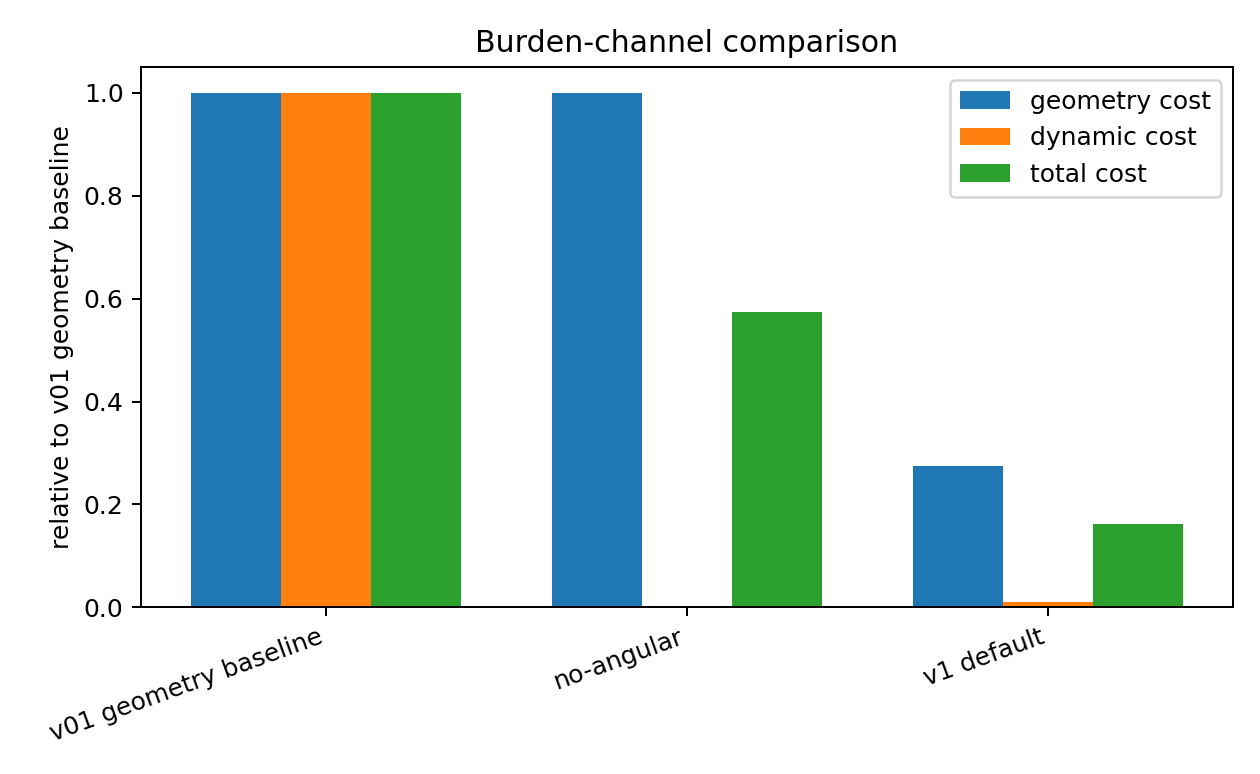
\includegraphics[width=0.74\linewidth]{../figures/burden_channel_comparison.png}
\caption{Burden-channel comparison. The balanced mixed-capacity design reduces geometry and dynamic channels together.}
\label{fig:burden_channel}
\end{figure}

\begin{figure}[H]
\centering
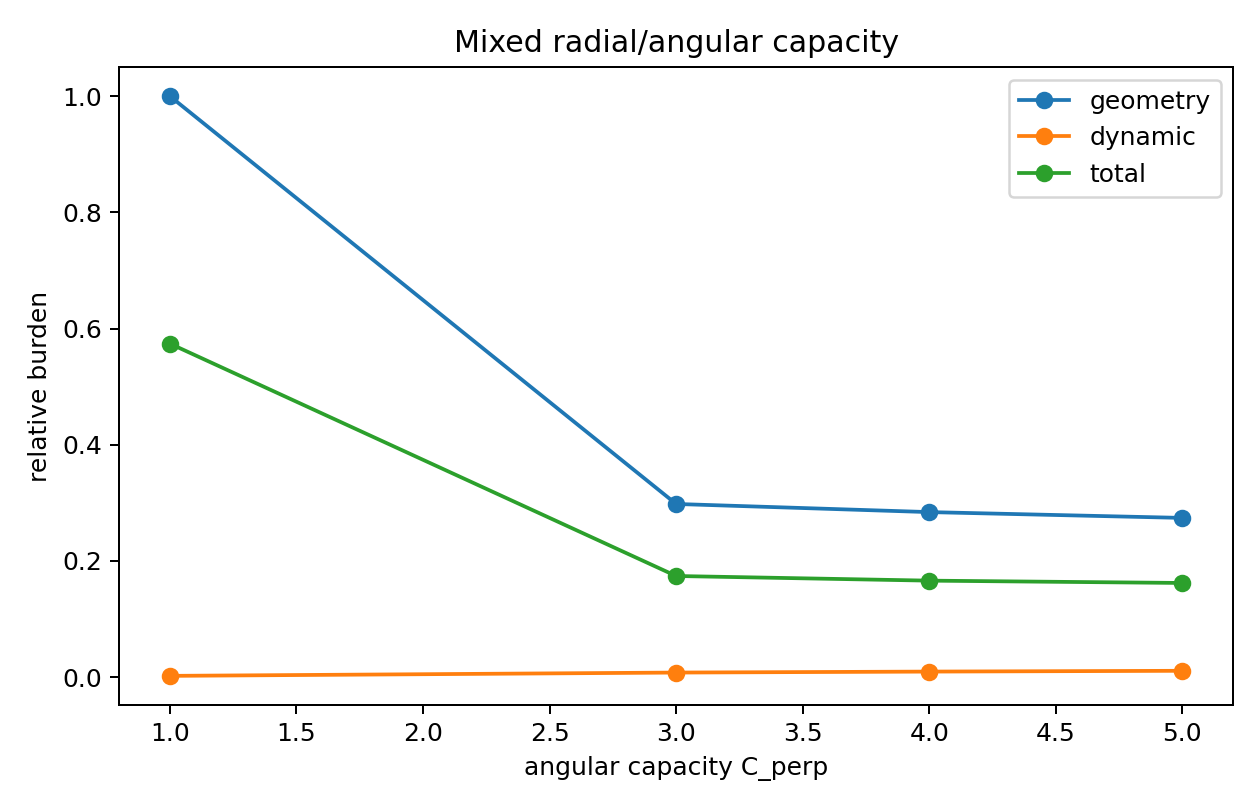
\includegraphics[width=0.74\linewidth]{../figures/mixed_capacity_comparison.png}
\caption{Mixed radial/angular capacity comparison. The radial-only branch is current-clean and geometry-heavy; moderate angular capacity reduces spatial burden.}
\label{fig:mixed_capacity}
\end{figure}

\begin{table}[H]
\centering
\caption{Geometry confirmation. Costs are relative to the reference geometry.}
\label{tab:geometry}
\begin{tabular}{lrrrr}
\toprule
Candidate & total & geometry & dynamic & packet norm \\
\midrule
reference geometry & 1.000 & 1.000 & 1.000 & -0.696 \\
radial-only $C_\perp=1$ & 0.574 & 1.000 & 0.00208 & -0.762 \\
$C_\perp=3$ branch & 0.174 & 0.298 & 0.00776 & -0.762 \\
$C_\perp=4$ branch & 0.166 & 0.284 & 0.00944 & -0.762 \\
balanced default $C_\perp=5$ & 0.162 & 0.274 & 0.0108 & -0.762 \\
reserve branch $C_0=100,C_\perp=5$ & 0.174 & 0.278 & 0.0341 & -0.766 \\
\bottomrule
\end{tabular}
\end{table}

\subsection{Source-exposure evidence}

\begin{figure}[H]
\centering
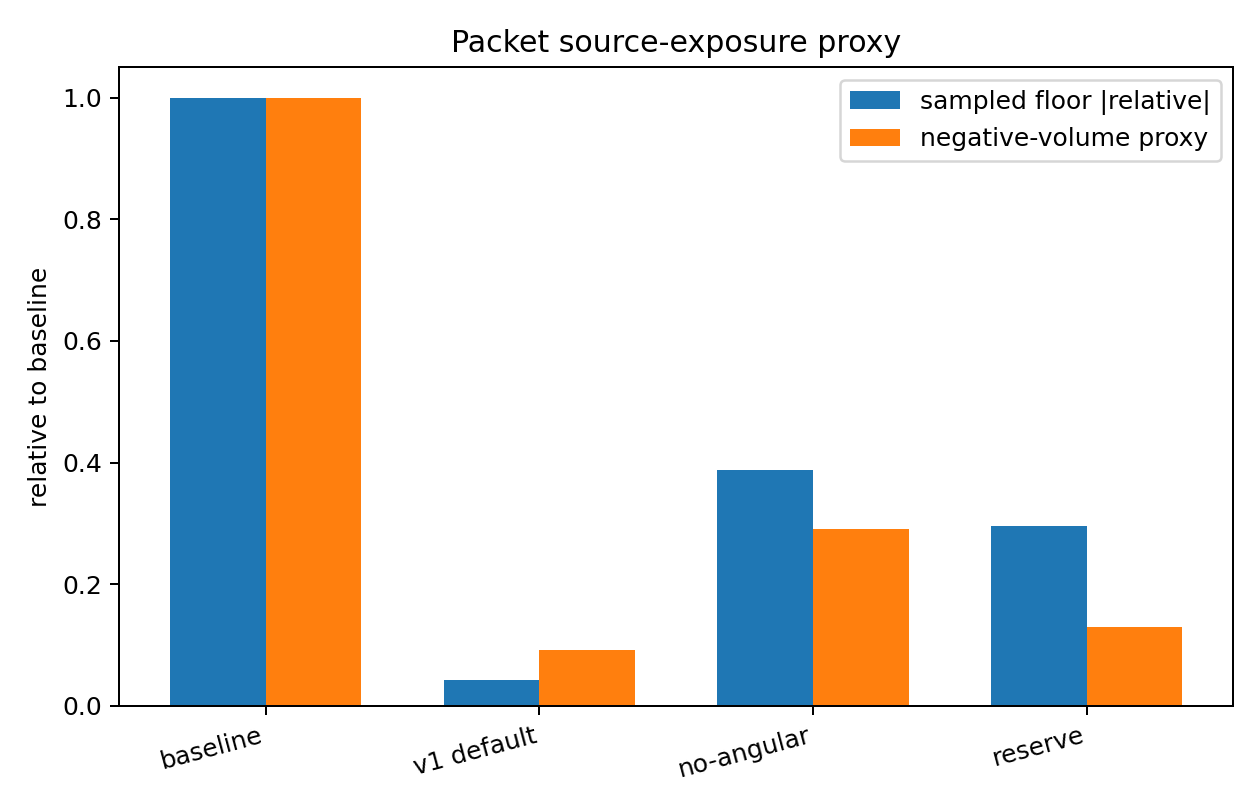
\includegraphics[width=0.74\linewidth]{../figures/packet_source_exposure.png}
\caption{Packet source-exposure proxy at $V=10$, $\lambda=6$. The balanced default reduces sampled packet exposure and negative-volume exposure relative to the reference geometry.}
\label{fig:packet_source_exposure}
\end{figure}

\begin{table}[H]
\centering
\caption{Conservative current-floor source screen at $V=10$, $\lambda=6$.}
\label{tab:source}
\begin{tabular}{lrrrr}
\toprule
Case & packet min floor & neg. volume rel. & $j_M$ rel. & Lorentzian floor rel. \\
\midrule
reference geometry & -0.789658 & 1.000 & 1.000 & 1.000 \\
balanced default $C_\perp=5$ & -0.124632 & 0.092 & 0.011 & 0.042 \\
radial-only $C_\perp=1$ & -0.319837 & 0.291 & 0.00134 & positive floor \\
reserve branch & -0.149332 & 0.130 & 0.046 & 0.295 \\
\bottomrule
\end{tabular}
\end{table}

\subsection{Robustness evidence}

\begin{table}[H]
\centering
\caption{Pressure-sensitive robustness screen at $61\times25$ grid in the stressed case. Values are relative to the reference geometry.}
\label{tab:robust_pressure}
\begin{tabular}{lrrrr}
\toprule
Case & total & geometry & dynamic & pressure exposure \\
\midrule
balanced default $C_\perp=5$ & 0.119 & 0.158 & 0.020 & 0.213 \\
pressure branch $C_\perp=3$ & 0.142 & 0.192 & 0.015 & 0.144 \\
radial-only $C_\perp=1$ & 0.721 & 1.000 & 0.005 & 0.026 \\
reference geometry & 1.000 & 1.000 & 1.000 & 1.000 \\
\bottomrule
\end{tabular}
\end{table}

\begin{figure}[H]
\centering
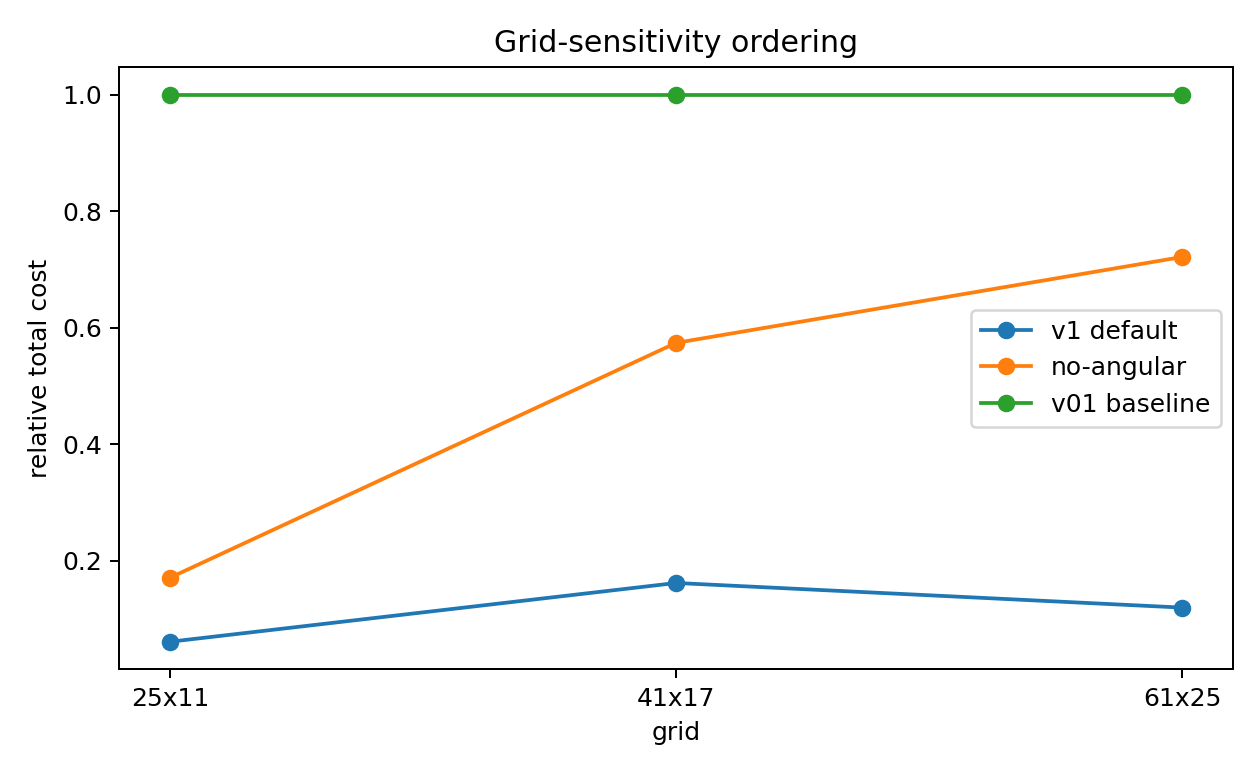
\includegraphics[width=0.74\linewidth]{../figures/grid_sensitivity.png}
\caption{Grid sensitivity. The mixed-capacity candidate preserves the ordering over the tested grids.}
\label{fig:grid_sensitivity}
\end{figure}



\section{How this reframes feasibility under source availability}

Under the source-availability assumption, feasibility becomes a question about placement, timing, and exposure. The support is admitted as an engineering input. The design question is where that support acts, what job it performs, and how directly the passenger packet samples it.

The frozen design answers that question by giving the burden a geography. The throat core supplies the active rail. The transition layer carries the current needed to catch the packet and fade the shift. The angular capacity sector relieves spatial-curvature concentration instead of leaving all capacity in the radial direction. The support edge contains the harshest infrastructure gradients. The packet worldtube becomes the cabin-level object whose sampled exposure can be screened separately from the plant.

This geography is the feasibility contribution. A source model built for the composite architecture receives separate source targets rather than a single undifferentiated exotic-matter demand. One target supports the throat. One target carries transition current. One target supplies angular capacity. One target manages shoulder matching and reset. One target protects the packet coupling. The reduced screens show how those targets move when the design is changed, and the frozen candidate selects the operating family where the packet remains clear while the spatial and current burdens are assigned to the plant.

The next research steps inherit that map. A pressure-complete stress tensor can be evaluated region by region. Constraint-quality data can preserve the same packet, edge, and support regions. Evolution tests can follow the catch, fade, and relax sequence as a service cycle rather than treating the geometry as a static object. Repeated-operation studies can ask how the plant resets and where source ledgers accumulate. The frozen design therefore gives future source construction a layout: where the source acts, which burden it carries, and how close that burden comes to the passenger packet.

\section{Source construction gates opened by the frozen design}

The frozen design gives the next source-construction problem a layout. The source is no longer a single symbolic object placed wherever the metric needs it. It becomes a set of regional jobs tied to the service cycle. The throat core supplies active rail support. The transition layer carries the current required to catch the packet and fade the shift. The angular capacity sector relieves spatial-curvature concentration. The shoulder and reset regions manage matching and recovery. The packet coupling region is the cabin-level target, where sampled exposure and tidal behavior matter most directly.

That layout changes how the next calculation should be organized. A pressure-complete stress tensor can be decomposed by role instead of reported only as a global field. The useful question becomes: which part of $T_{\mu\nu}$ supports the throat, which part carries transition current, which part supplies angular capacity, which part manages shoulder matching, and which part reaches the packet? The current-floor screen already points to that decomposition. It shows that the packet channel can be improved more strongly than the total source-demand norm, because the design suppresses the current term that the packet samples most sharply.

The same layout guides constraint-quality initial data. The packet, support edge, transition layer, and shoulder region are distinct places with distinct jobs. Constraint solving can preserve that geography. It can test whether the mixed-capacity operating band still separates the current channel from the curvature channel when the reduced prescribed metric is replaced by higher-fidelity initial data.

The evolution problem inherits the service cycle. The meaningful perturbation is not only a ripple in a static geometry; it is a disturbance during catch, fade, relaxation, and reset. A stable design keeps the packet protected while the plant changes state around it. Repeated operation then becomes a ledger question: where do source histories accumulate, how cleanly does the support edge reset, and how much margin remains when the plant cycles again?

The chronology problem also becomes more concrete. A network of such systems would need scheduling rules for active plants, not just geometric rules for connected mouths. The service packet, throat plant, support edge, and reset interval give chronology analysis operational handles. They identify the moments when the system is open, coupled, relaxing, and unavailable.

These gates are demanding, but they are now attached to a specific architecture. The frozen design gives future work a map of where to look and what each region is supposed to do.

\section{Conclusion}

The Catch-Rematched Hybrid Flare-Gated Transit v1 design presents a source-supplied spacetime service architecture. The throat is active rail infrastructure. The passenger rides a protected packet. The transport field couples the packet to the throat plant during a controlled service sequence: support is prepared, capacity is supplied, the packet is caught, the shift fades, the throat relaxes, and the plant resets.

The central result is the distribution of burden. Packet safety, infrastructure accessibility, transition-current control, capacity support, spatial-curvature management, and recovery are separate engineering channels. The packet norm measures the passenger environment. Stationary $g_{tt}$ measures infrastructure accessibility. Momentum-current and extrinsic-curvature proxies identify transition burden. Hamiltonian and spatial-curvature proxies identify capacity/support burden. The frozen candidate assigns these roles to distinct parts of the plant instead of asking one geometric region to do every job.

The design's most informative features are the ones that create this separation. Catch/rematch choreography protects the packet through shift release. Medium transition widths and $W^4$ edge shaping reduce the current and extrinsic-curvature channel. Mixed radial/angular capacity reduces spatial-curvature concentration. The balanced default uses moderate angular capacity as a curvature-management actuator, with a nearby pressure/current-leaning branch. The source screen then shows the architecture doing its intended work: packet current-floor exposure falls much more sharply than the total source-demand proxy alone would suggest, because the design cleans the channel that the packet samples.

This is the field contribution. The standard literature identifies the pressures that make macroscopic FTL geometries hard: exotic support, quantum-inequality severity, thin walls, capacity bookkeeping, ADM role coupling, prepared-route control, and source timing. The frozen design shows how those pressures can be arranged inside a composite wormhole/warp service system. It gives the burden a geography and a sequence. It tells future source models where support acts, what each source channel carries, and how close each burden comes to the passenger packet.

The next stage is source construction on that map. Pressure-complete stress evaluation, quantum-inequality screening, constraint-quality initial data, evolution, repeated operation, and chronology analysis can now be organized around the same service roles: throat support, transition current, angular capacity, shoulder/reset matching, and packet coupling. The v1 design is therefore a frozen reduced target for the next physics layer: an active throat plant carrying a protected packet through a managed spacetime service cycle.

\bibliographystyle{unsrtnat}
\bibliography{references}

\end{document}
